Consider the following class diagram candidates:

\figureSeriesHere{}{\figureSeriesRow{\figureSeriesElement{1}{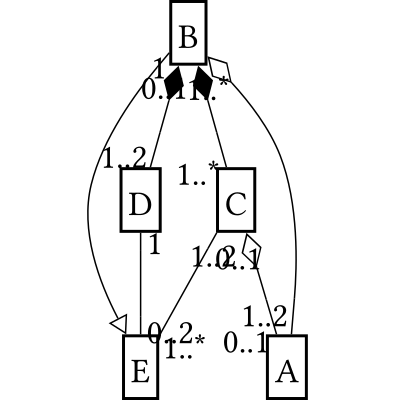
\includegraphics[min width=0.5\textwidth,min height=0.4\textwidth,max width=\textwidth,max height=\textwidth]{52/cd0ebeaa4263d7a751b1afb99e514b70e073b89f9719329160cf057c33fb6e111f00af83b04c596701db35357ce8aed00a3a92e08161.pdf}}}\figureSeriesRow{\figureSeriesElement{2}{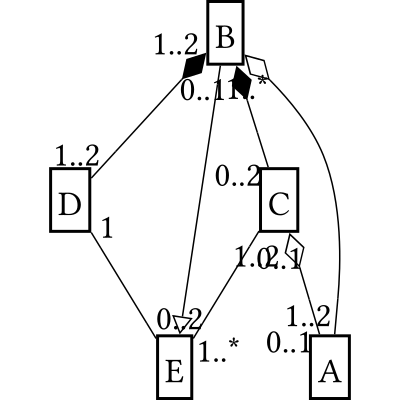
\includegraphics[min width=0.5\textwidth,min height=0.4\textwidth,max width=\textwidth,max height=\textwidth]{52/cd7a8aec498e74a41320385551bd1abc5613be2814f2815896df755298e5df2aed00af83b04c596701db35357ce8aed00a3a92e08161.pdf}}}\figureSeriesRow{\figureSeriesElement{3}{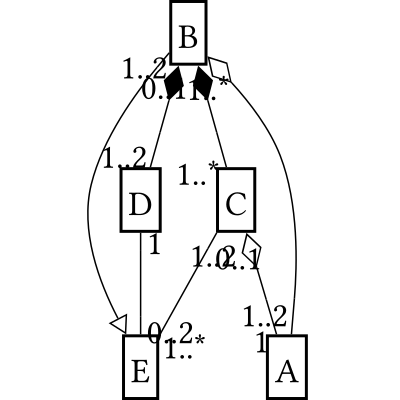
\includegraphics[min width=0.5\textwidth,min height=0.4\textwidth,max width=\textwidth,max height=\textwidth]{52/cdbb94aeaa70e6e2bba23762be906eba6c07a58494f0038c6902b3ecf93df0d24200af83b04c596701db35357ce8aed00a3a92e08161.pdf}}}\figureSeriesRow{\figureSeriesElement{4}{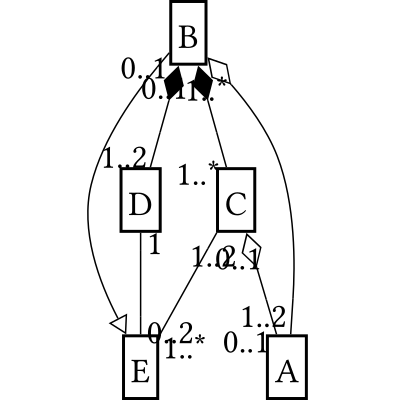
\includegraphics[min width=0.5\textwidth,min height=0.4\textwidth,max width=\textwidth,max height=\textwidth]{52/cdd98fa5f9699f7f24fc7953cf62b89e3298c6ff397cc23315cb8f3389b466b03200af83b04c596701db35357ce8aed00a3a92e08161.pdf}}}}Which of these class diagram candidates are valid class diagrams?
Please state your answer by giving a list of numbers, indicating all valid class diagrams.

For example,
\begin{minted}{text}
[1, 2]
\end{minted}
would indicate that only class diagram candidates 1 and 2 of the given ones are valid class diagrams.

Please note: Classes are represented simplified here. 
 That means they consist of a single box containing only the class name but no sections for attributes or methods. 
 Nevertheless you should treat these simplified class representations as valid classes.

Please note: When hovering over or clicking on edges / nodes or their labels, the respective components that belong together are highlighted.

